%!TEX root = ../../report.tex
\section{The Dynamic Mapping on MiR-100}
In the test platform used in this project the output required by the subscribing systems is a costmap. This grid represents the world as cells, each with a value for the cost of traversing it. 
The system is built to be run with the MiR-100 robot. This involves constructing and interfacing the Dynamic mapping system with the ROS setup on the robot. The developed system is shown in figure \ref{fig:mir_interface} along with the ROS nodes it interacts with. 

\begin{figure}[htbp]
	\centering
	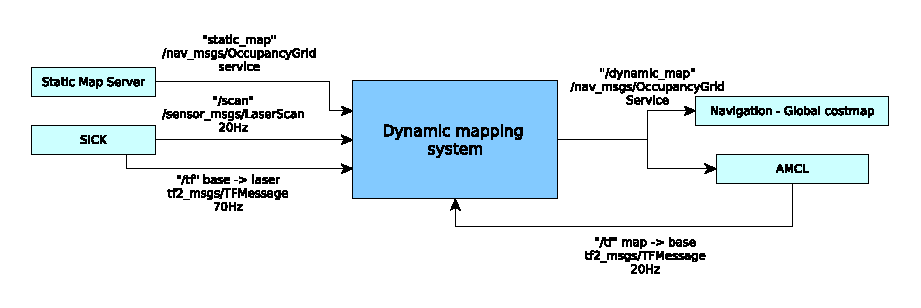
\includegraphics[width=1\linewidth]{chapters/cost_interpretation/figures/dynamic_map_mir_interface.eps}
	\caption{The Dynamic mapping system with connected nodes and interface.}
	\label{fig:mir_interface}
\end{figure}

The Dynamic mapping system receives a static map from the Static Map Server in order to initialize the Dynamic learner. This is only done at startup. The primary input for the Dynamic mapping system is the laser scan data provided by the SICK node and the pose of the robot in the world provided by AMCL. The pose of the scanners on the robot is provided by the SICK system. 
The Dynamic mapping system is based on the ROS implementation of the Layered costmap \cite{lu2014layered}. Each layer maintains its own costmap and these are combined to produce the output costmap. Figure \ref{fig:dynamic_map_server_internal} shows the elements of the Dynamic mapping system and the flow of data. The layered costmap in the Dynamic mapping system contains three layers; Activity, User priority and Blueprint layer. 

\begin{figure}[htbp]
	\centering
	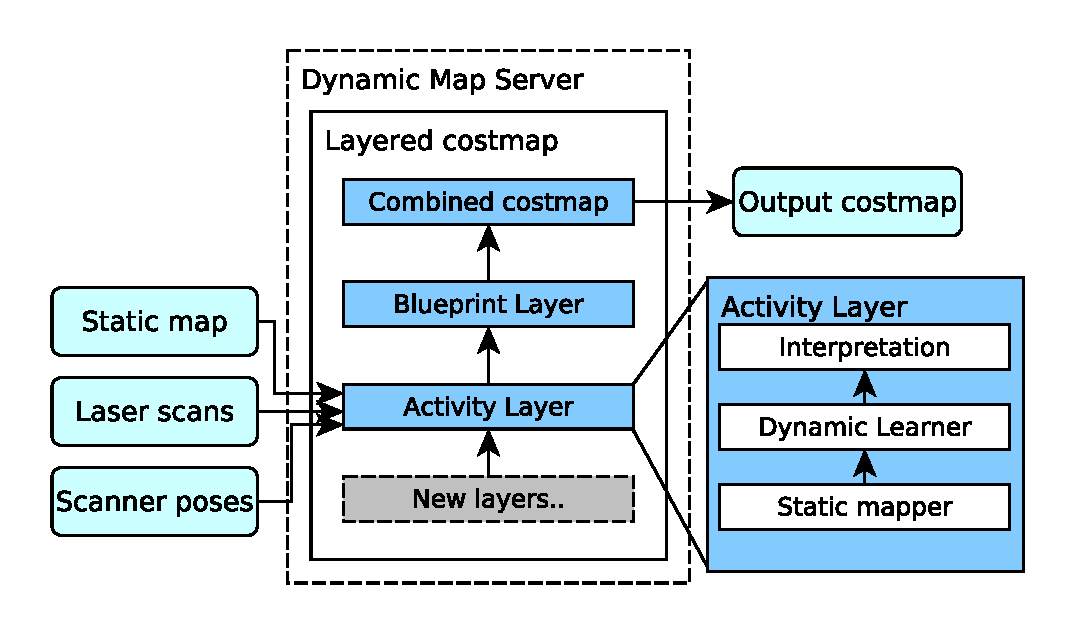
\includegraphics[scale=0.7]{chapters/cost_interpretation/figures/implementation_overview.eps}
	\caption{The Dynamic Map Server internal components}
	\label{fig:dynamic_map_server_internal}
\end{figure}

The Activity Layer is the primary layer and handles the mapping, learning of the dynamics and interpretation of the dynamics in three sections. 
The sections are implemented to enable easy replacement.
Particularly the Static mapper is loosely coupled to the Dynamic learner.
This is done by having a well defined interface between the sections which allows changing the Static mapper and Dynamic learner separately.
It delivers a costmap that should contain the learned static obstacles with a high cost and dynamic obstacles with a cost appropriate to its dynamic.
 

The second layer in the Dynamic Map Server is the User priority layer. This layer is designed override the cost of certain cells. This could be used to ensure that selected areas are avoided or preferred based on the user requirements. 

The Blueprint layer can contain walls and structural elements of the environment.
These elements are expected to be absolutely stationary for the entire time of operation.
This can be used to avoid any possible erosion, of the walls in the map representation, due to erroneous localization.
Another benefit of the Blueprint layer is to limit the risk of unintended feedback by wrong mapping due to  erroneous localization.
The Blueprint layer is implemented as an instantiation of the Static Map Layer \cite{lu2014layered}. 

Because the Dynamic mapping system is implemented as a layered costmap it is possible add new layers by means of a simple ROS API \cite{plugin_lib}. This could be layers for other sensors, like SONAR \cite{range_sensor_layer} or 3D cameras.
